\section{はじめに}

タンパク質はアミノ酸が多数繋がって構成されている高分子化合物であり、タンパク質全体が分子機械として働く。しかしこのアミノ酸単位やアミノ酸間の相互作用という”部分”としての局所的挙動とドメイン単位やタンパク質という”全体”としての大域的挙動には時空間の大きな隔たりがある。
それが顕著に表れている具体的な話でいうと、タンパク質のアロステリー現象が挙げられる。
タンパク質のアロステリー現象は、リガンド結合や外部刺激によって生じる構造変化が刺激受容部位から遠隔の活性部位に影響を及ぼす現象であり、そのメカニズム解明は生命現象の理解と創薬研究の中心的的題の一つである。
%参考文献:アロステリーの特性
%2009「アロステリーと協同性の再考」
%https://onlinelibrary.wiley.com/doi/10.1110/ps.03259908
アロステリーはタンパク質の機能を制御する重要な特性であり\cite{Cui2009}、リガンド結合など外部刺激のシグナルが残基間相互作用を介して活性部位に伝達する仕組みを提供する。
この過程の特徴を2点挙げる。\\
1.活性部位がサブÅ~数十Å離れた場所でのリガンド結合や微小環境の摂動を総じた情報を受け取る点。\\
2.ピコ秒オーダーの残基間エネルギー移動過程\cite{Lim1996}がミリ秒以上のアロステリック遷移\cite{Changeux2005}を引き起こす点。
つまりこの過程は、サブピコ秒からミリ秒の時間スケールにわたるダイナミクスと、サブÅから数十Åの空間スケールの相互作用が連動して行われることが興味深い点であり大きな謎\cite{Fenton2008}となっている。
%参考文献:アロステリー、時間スケールと空間スケール
%2005「シグナル伝達のアロステリック機構」
%https://www.science.org/doi/abs/10.1126/science.1108595
%大きな謎
%2008「アロステリー:「生命の第二の秘密」の図解による定義」
%https://www.sciencedirect.com/science/article/pii/S0968000408001643
この離れた場所間のコミュニケーションを解明する一つの方法として、グラフ理論\cite{Zhou2018}を用いたアプローチが注目されている。
%参考文献:グラフ理論
%https://pubs.acs.org/doi/10.1021/acs.chemrev.7b00305
グラフ理論は、分子内の残基間の相互作用をネットワークとして表現し、複雑な動的挙動を解析するための強力なツールとして広く利用されてきた\cite{Doncheva2011}\cite{Martin2011}\cite{Doncheva2012}。
%参考文献:グラフ理論
%2011「タンパク質構造の残基ネットワークの解析と可視化」
%https://www.cell.com/trends/biochemical-sciences/abstract/S0968-0004(11)00013-2?_returnURL=https%3A%2F%2Flinkinghub.elsevier.com%2Fretrieve%2Fpii%2FS0968000411000132%3Fshowall%3Dtrue
%2011「RING: タンパク質構造における相互作用残基、進化情報、エネルギーのネットワーク化」
%https://academic.oup.com/bioinformatics/article/27/14/2003/193801?login=false
%2012「生物学的ネットワークとタンパク質構造のトポロジー解析とインタラクティブな可視化」
%https://www.nature.com/articles/nprot.2012.004
タンパク質を構造ネットワークとしてモデル化すると、シグナル伝達機構を解釈しやすくなる。
そのようなモデルは、ネットワーク内の最短経路の存在の重要性を強調\cite{Ghosh2007}しており、それらが離れた部位間での効率的な情報伝達に寄与していることを示している。
%参考文献:最短経路
%2007「分子動力学シミュレーションと構造ネットワーク解析によるメチオニルtRNA合成酵素のコミュニケーション経路の研究
%https://www.pnas.org/doi/full/10.1073/pnas.0704459104
また、その前提のもとで、高い中心性を持つ残基\cite{amitai2004}やネットワーク上における最短経路上によく現れる残基\cite{delsol2006}を解析することで、機能的残基を同定してきた。
%参考文献:中心性
%2004「タンパク質構造のネットワーク解析により機能残基を特定」
%https://www.sciencedirect.com/science/article/pii/S0022283604013592
%参考文献:最短経路
%2006「ネットワーク通信における短い経路を維持するために重要な残基がタンパク質のシグナル伝達を媒介する」
%https://www.embopress.org/doi/full/10.1038/msb4100063
実際にこれらの残基はタンパク質の折りたたみにおける重要なアミノ酸や酵素ファミリーの活性部位残基であると関連付けられている。

しかし、残基間エネルギー移動過程とアロステリック遷移の時間スケールの違いを考慮すると、単純な「最短経路モデル」だけではアロステリーの情報伝達を十分に説明できない可能性がある。
実際に、残基集団の協調的な運動\cite{Kornev2015}や、複数経路の存在\cite{delSol2009}を示す文献もあり、この視点はアロステリーのより現実的で包括的な理解を提供する可能性がある。
%複数経路の論文
%2009「アロステリック機能調節の起源:複数の既存経路」
%https://www.sciencedirect.com/science/article/pii/S0969212609002500?via%3Dihub
%参考文献:バイオリンモデル
%2015「タンパク質キナーゼにおけるダイナミクス駆動型アロステリー」
%https://www.cell.com/trends/biochemical-sciences/fulltext/S0968-0004(15)00166-8

本研究では、アロステリーの解析対象として$\beta_2$アドレナリン受容体($\beta_2$AR)を選定した。
まず分子動力学(MD)シミュレーションを用いて得られたinactive状態とactive状態におけるトラジェクトリー解析から、残基間距離を反映したネットワークを構築した。
さらに、Louvain法\cite{Blondel2008}によるコミュニティ検出を適用し、コミュニティによるシグナル伝達機構を定量的に解析した。

その結果、active状態において新たなコミュニティの生成が有意に認められ、これがシグナル伝達において重要な役割を果たすことが示唆された。
また、膜タンパク質内のエネルギー的に保存された水分子\cite{Angel2009}が果たす役割を確認した。

\section{$\beta_2$アドレナリン受容体($\beta_2$AR)}
\label{sec:b2ar}

\subsubsection{基本情報}
$\beta_2$アドレナリン受容体($\beta_2$AR)は、Gタンパク質共役受容体(GPCR)の一種である。
GPCRは細胞膜に存在する膜タンパク質であり、ホルモンや神経伝達物質などの細胞外刺激を認識し、それを細胞内のシグナルに変換する役割を担っている。
また、視覚、嗅覚、味覚といった感覚にも関与し、生体内の多様なシグナル伝達経路において中心的な役割を果たしている。
GPCRは7回膜貫通構造を持つことが特徴であり、各膜貫通ヘリックス(TM1からTM7)は、細胞外ループ(ECL)と細胞内ループ(ICL)を介して他のヘリックスと連結されている。
この構造により、細胞外でのリガンド認識と細胞内でのシグナル伝達を効率的に行うことが可能となる。

%TM1-7
\begin{figure}[htbp]
  \centering
  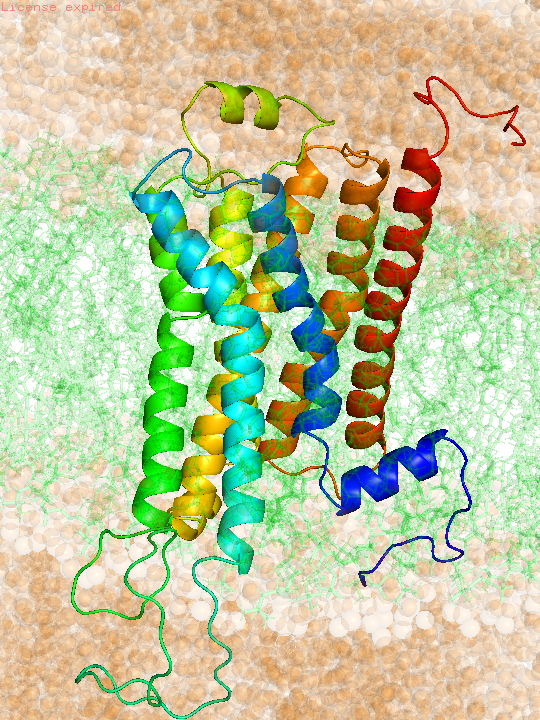
\includegraphics[width=0.8\textwidth]{system-all.png}
  \caption{$\beta_2$ARの膜貫通ヘリックス。}
  \label{fig:all}
\end{figure}

\newpage

膜タンパク質の構造データは、Protein Data Bank(PDB)から取得した。
$\beta_2$ARの不活性状態として2RH1\cite{cherezov2007},活性状態として3P0G\cite{rasmussen2011}を用いた。
%2RH1の構造情報2007
%https://www.science.org/doi/10.1126/science.1150577
%3P0Gの構造情報2011
%https://www.nature.com/articles/nature09648

\subsubsection{活性化に伴う構造的変化}
$\beta_2$ARのinactive状態からactive状態への活性化は、リガンド結合部位に結合したアゴニストによって引き起こされる。
すると受容体が活性化され、特にGsといったGタンパク質の結合が促進される。
Gsはヘテロ三量体型タンパク質であり、その活性化により細胞内でアデニル酸シクラーゼが刺激され、cAMP(サイクリックAMP)の産生が増加する。
この過程\cite{philip2007}を通じて、細胞内のシグナル伝達経路が活性化される。
%参考文献:GPCRのシグナル伝達機構
%2007「G タンパク質共役受容体とそれに対応する G タンパク質を介したシグナル伝達は、化学量論的に制限されたモデルに従う」
%https://www.sciencedirect.com/science/article/pii/S002192582087389X

%詳細の構造と、リガンド・gタンパク質結合部位を示す
β2ARのリガンド結合部位は膜貫通ヘリックス(TM)の間に位置し、細胞外の刺激を感知する。
一方で、Gタンパク質との結合は細胞内ループおよび細胞質側ドメインを介して行われる。


\subsubsection{活性化に関わる重要な残基}
$\beta_2$ARの活性化において、特定のモチーフ\cite{nygaard2009ligand}\cite{lee2013mapping}
が重要な役割を果たしていることが知られている。

%参考文献:モチーフ
%2009「7TM受容体構造におけるリガンド結合とマイクロスイッチ」
%https://www.sciencedirect.com/science/article/pii/S0165614709000546
%参考文献:モチーフ
%2013「Gタンパク質共役受容体の分子内シグナル伝達のマッピング」
%https://onlinelibrary.wiley.com/doi/10.1002/prot.24451
%参考文献:保存水
%2009「保存された水はファミリーA(ロドプシン様)Gタンパク質共役受容体の構造的および機能的活性化を媒介する」
%https://www.pnas.org/doi/10.1073/pnas.0903545106
モチーフとは、タンパク質中の特定の機能に関連する保存されたアミノ酸配列のことであり、GPCRではアロステリックシグナル伝達やコンフォメーション変化を介して受容体の機能を調節する。
$\beta_2$ARを含むクラスA GPCRでは、以下の4つの主要な保存モチーフ(DRY、CWxP、NPxxY、PIF)と「イオンロック」が重要な役割を果たしている。

\begin{itemize}
  \item \textbf{DRYモチーフ}  
  TM3の細胞質側領域に位置し、Asp(D)-Arg(R)-Tyr(Y)から構成される。inactive状態ではTM6のGluとイオンロックを形成し、構造を安定化させている。一方、active状態ではイオンロックが解除され、Gタンパク質との結合が可能になる。

  \item \textbf{CWxPモチーフ}  
  TM6のリガンド結合ポケットの底部に位置し、Cys(C)-Trp(W)-任意の残基(x)-Pro(P)から構成される。inactive状態ではTrpがリガンド結合ポケットを開いた状態を維持しているが、active状態ではTrpが「トグルスイッチ」として機能し、ポケットを閉じる役割を果たす。

  \item \textbf{NPxxYモチーフ}  
  TM7の細胞質側に位置し、Asn(N)-Pro(P)-任意の残基(xx)-Tyr(Y)から構成される。このモチーフにおけるTyrは、不活性状態と活性状態で異なる立体配座間を回転することで、構造の変化を媒介する。

  \item \textbf{PIFモチーフ}  
  TM4、TM5、TM6にまたがる位置に存在し、Pro(P)-Ile(I)-Phe(F)から構成される。このモチーフにおけるPheはスイッチとして機能し、活性化時に異なる立体配座間で方向を変えることで重要な役割を果たす。

  \item \textbf{イオンロック}  
  TM3とTM6の間に位置している。不活性状態ではイオンロックが形成され、構造を安定化させているが、活性化時にはこのロックが解除され、GPCRの完全な活性化を促進する。
\end{itemize}


また水分子も、生物学的システムにおいて重要な役割を果たすことが知られており、特にGPCRの活性化メカニズムにも深く関与している。
ロドプシンをはじめとするGPCRにおいて、保存された水は活性化過程においてアロステリックを仲介する機能を果たすことが示されている\cite{angel2009conserved}。
$\beta_2$ARにおいても、膜貫通ドメイン内にはいくつかの保存された水分子が確認され、これらの水分子はアロステリックシグナル伝達に関与していると考えられる。
らに、inactive状態とactive状態それぞれのβ2AR構造間で水分子の位置や配置がどのように変化するかを比較することで、水の動態が受容体の機能に与える影響を明らかにすることができる可能性がある。

そこで本研究でも、モチーフと保存された結晶水がコミュニティ構造に与える影響を解析し、シグナル伝達機構における役割を明らかにすることを目指す。
